\documentclass[conference]{IEEEtran}
\IEEEoverridecommandlockouts
% The preceding line is only needed to identify funding in the first footnote. If that is unneeded, please comment it out.
\usepackage{cite}
\usepackage{amsmath,amssymb,amsfonts}
\usepackage{algorithmic}
\usepackage{graphicx}
\usepackage{textcomp}
\usepackage{xcolor}
\usepackage{url}
\usepackage{soul}
\usepackage{multirow}
\usepackage{lmodern}
\usepackage{framed}
\usepackage{color}
\usepackage{booktabs}
\usepackage{anyfontsize}

\def\BibTeX{{\rm B\kern-.05em{\sc i\kern-.025em b}\kern-.08em
    T\kern-.1667em\lower.7ex\hbox{E}\kern-.125emX}}
\begin{document}
\nocite{*}

\title{Conference Paper Title*\\
% {\footnotesize \textsuperscript{*}Note: Sub-titles are not captured in Xplore and
% should not be used}
% \thanks{Identify applicable funding agency here. If none, delete this.}
}

\author{
\IEEEauthorblockN{Elie Neghawi}
\IEEEauthorblockA{\textit{Electrical and Computer Engineering} \\
\textit{Concordia University}\\
Montreal, Canada \\
e\_negh@encs.concordia.ca}

\and

\IEEEauthorblockN{Yan Liu}
\IEEEauthorblockA{\textit{Electrical and Computer Engineering} \\
\textit{Concordia University}\\
Montreal, Canada \\
yan.liu@concordia.ca}
}

\maketitle

\begin{abstract}
	Adoption of AI systems has been widely used across multiple industry domains at an alerting rate without the focus on it's ethical concerns. To address those concerns, there are an increase number of AI ethics frameworks that have been suggested recently that focus on the algorithmic level rather on the systems level. Nonetheless, some of the system level approaches developed mostly cover a single level governance pattern of the system components in the entire software design lifecycle. However, the need to go beyond the single level  system design AI ethics frameworks to allow not only a better responsible-AI-by-design, but also a trustworthy process patterns that abstract and link the underlying layers of responsible AI on each and every level. This paper illustrates a principal-to-practice guide of the multi-level governance (MLG) within organizations across the globe for AI ethics frameworks. We outline the main areas of gap in organizations for AI ethics frameworks. Consecutively, we propose a MLG pattern for responsible AI systems within organizations which is participatory, iterative, flexible and operationalizable that target those main gap areas. Finally, to assist practitioners to apply the multi-level governance AI in organizations and the impact that it has on the industry level, we will translate into effective and responsible AI practices using two case studies.
\end{abstract}

\begin{IEEEkeywords}
AI, AI ethics, trustworthy AI, AIMLOps, AIOps, software engineering, software architecture, pattern, best practice
\end{IEEEkeywords}

\section{Introduction}
Aritificial Intelligence (AI) reshaped our lives, helped people make better predictions and take more informed and wise decisions. However, these high tech are still in there infancy, and there remains much promise for AI to promote innovation and address global challenges that people face.

Consecutively, ethical concerns and anxieties are fuelling around AI \cite{DBLP}. There are lots of enquiries on the trustworthiness and adoption of AI systems, including concerns about exacerbating inequality, digital divide, climate change and market concentration. Additionally, there are concerns that the use of AI may compromise human rights and values such as privacy. To address these concerns and ensure the responsible development and use of AI, a collaborative effort involving multiple stakeholders and international cooperation issued guidelines and ethical principles. Despite the creation of ethical guidelines for AI development inside organization, it can be challenging for developers to apply these principles in practical situations. These principles are often abstract and may not provide clear direction for specific implementation \cite{abs-2111-09478}. Therefore, more specific and actionable guidelines are needed to assist developers in implementing ethical considerations in their AI systems. It is important to bridge the gap between ethical principles and the algorithms used in AI systems to ensure responsible development. However, The architecture of an AI ecosystem consists of three layers: AI software supply chain, AI system, and operation infrastructure. It is challenging to show the contribution of each.

One work that was proposed is Responsible AI Pattern Catalogue \cite{catalogue}, which takes a pattern-oriented approach to promoting responsible AI in practice. Instead of solely focusing on ethical principles or AI algorithms, this catalogue focuses on design patterns that practitioners can apply to ensure that their AI systems are responsible throughout the software development process. The catalogue is organized into three categories: 1) governance patterns to establish multi-level governance (MLG), 2) process patterns to establish trustworthy development processes, and 3) product patterns to integrate responsible design into AI systems. In addition, it focuses on all aspect of the ecosystem (Industry-level, Organization-level and Team-level) without the planning of the design and the developement tools to support the navigation and utilisation of the Responsible AI pattern catalogue.

\begin{figure*}[htbp!!]
	\centering
	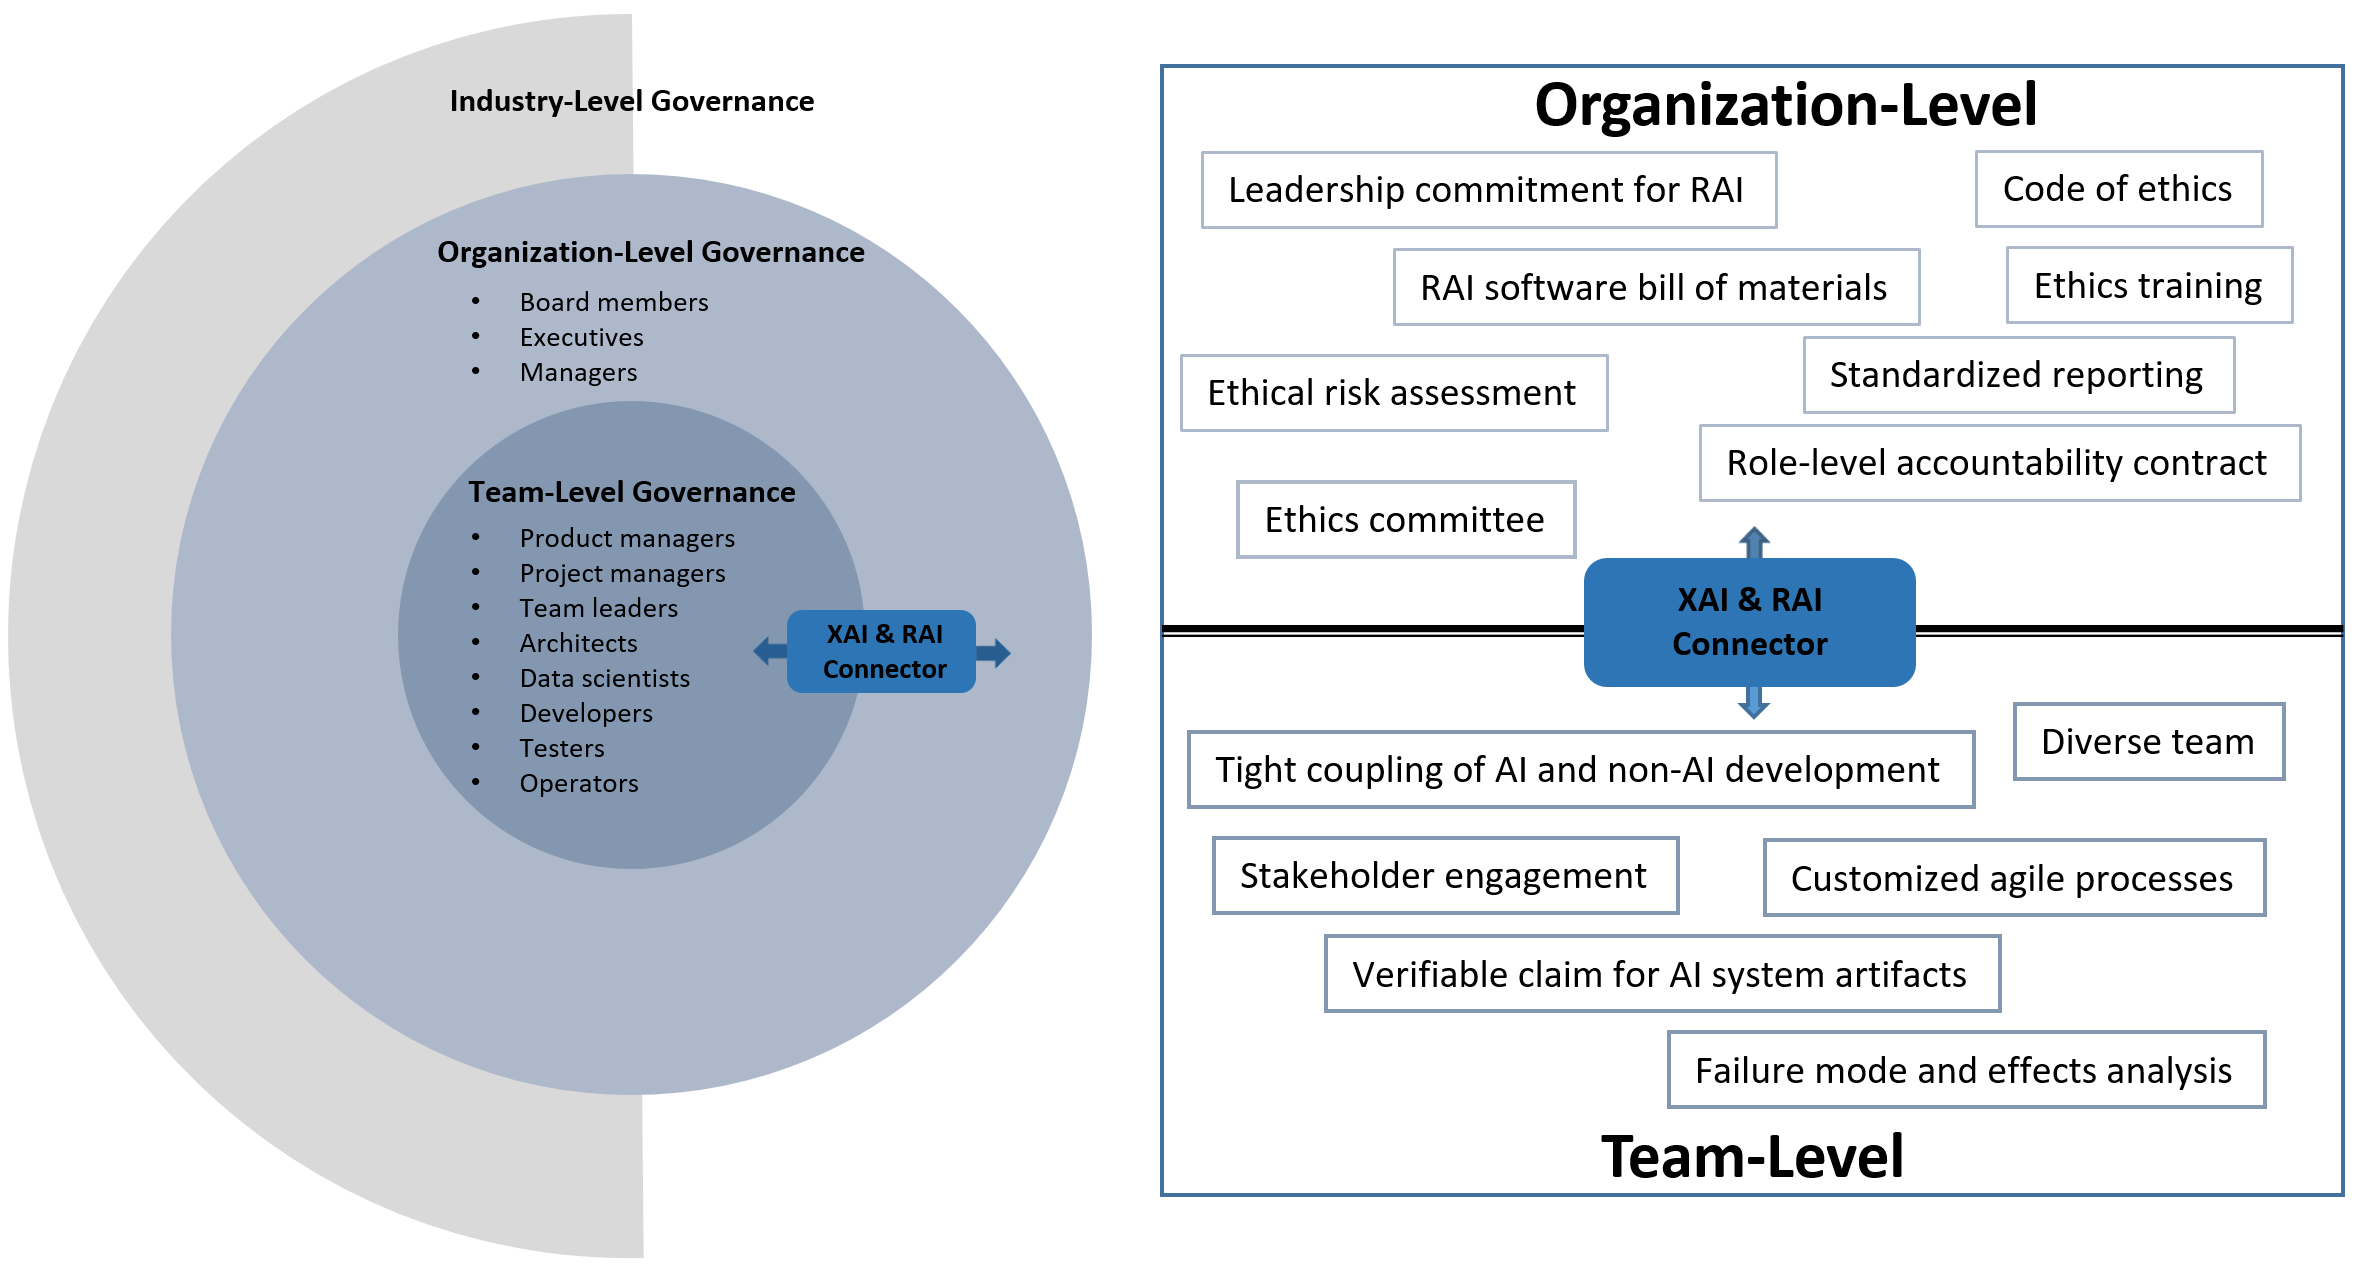
\includegraphics[width=0.8\textwidth]{Organization.png}
	\caption{Transition from traditional to the current approach}
	\label{ReMixMatch}
\end{figure*}
In this paper, we take a different approach by focusing on the organization-level patterns at the system level rather than just the ethical principles or AI algorithms. This approach aims to integrate responsible design in organizations into final AI products by looking at the bigger picture and the design patterns that shape the system as a whole. This is done with the intention of bridging the gap between the organizational-level and team-level and facilitating navigation. We start off by looking at the main two levels of an organization with the addition to the team-level and examine the current available methods \cite{Shneiderman, ShneidermanRespo, Jana, Hussain, roadmap}. Then we make the links on where those methods meets and create the best practices using the MLG patterns at the organization level. The overarching research question that has guided this study is:

% \begin{figure*}[h!]
% 	\centering
% 	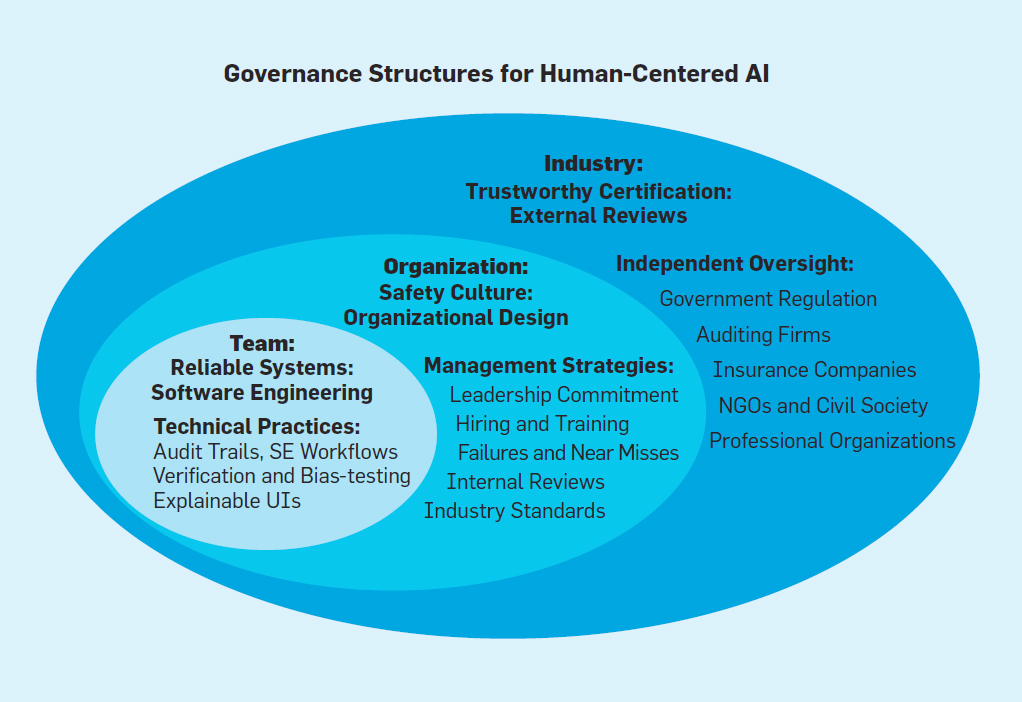
\includegraphics[width=4.74in]{governance.jpeg}
% 	\caption{Transition from traditional to the current approach}
% 	\label{ReMixMatch}
% \end{figure*}

\vskip 0.1in
\vskip 0.1in

\noindent\fbox{%
    \parbox{.48\textwidth}{%
     What is the multi-level governance pattern principle-to-practice proposed for responsible AI systems to bridge the gap between team-level and organization-level?}%
}

\vskip 0.1in
\vskip 0.1in

The main contributions of this paper are as follows:
\begin{itemize}
\item Find the link between Team-level governance patterns with the Organization-level patterns.
\item Suggest navigation and utilisation Team-level governance patterns with the Organization-level patterns.
\item Explore two case study that suits this principle-to-practice multi-level governance pattern.
\end{itemize}
\smallskip

To achieve responsible AI, there have been nearly 100 high-level AI ethics principles and guidelines issued by governments, organizations, and companies
\section{Related Work}
The issue of creating AI that is ethically accountable has garnered a great deal of interest among both industrial and academic communities. To promote ethical AI practices, a multitude of AI ethics principles and guidelines numbering around 100 have been established by various entities including governments, companies, and organizations. However, these guidelines are often too general and theoretical for individuals involved in the implementation of AI systems to apply in real-world scenarios.

There has been a concerted effort in the field of AI to address the challenges of responsible AI. One approach that has gained traction is the development of algorithm-level solutions. These solutions are designed to address specific aspects of the numerous high-level AI ethics principles and guidelines that have been established by various entities. By focusing on a subset of the principles, these algorithmic solutions aim to bring concrete and practical approaches to address some of the ethical concerns related to AI.

However, it's important to note that these algorithm-level solutions are just one part of the larger picture of responsible AI. Implementing them alone may not be enough to address all the ethical concerns related to AI, as the principles themselves are often complex and multifaceted. It requires a collaborative effort between researchers, developers, policymakers, and other stakeholders (board members, executives, managers) to ensure that AI is developed and used in an ethical and responsible manner.
\section{Methodology}
To best to our knowledge there is no standard for implementing the Multi-Level Governance (MLG) pattern for responsible AI systems with eXplainable AI (XAI). However, organizations can benefit from incorporating XAI technologies, such as interpretability and transparency tools, into their MLG processes to enhance the transparency and accountability of AI systems.

To build up the links of the multi-level governance for responsible AI systems within organizations, we performed a systematic combinations of organization-level and team-level governance to collect patterns. Figure illustrates the transition from the traditional approach to the new approach.

\begin{figure*}[h!]
	\centering
	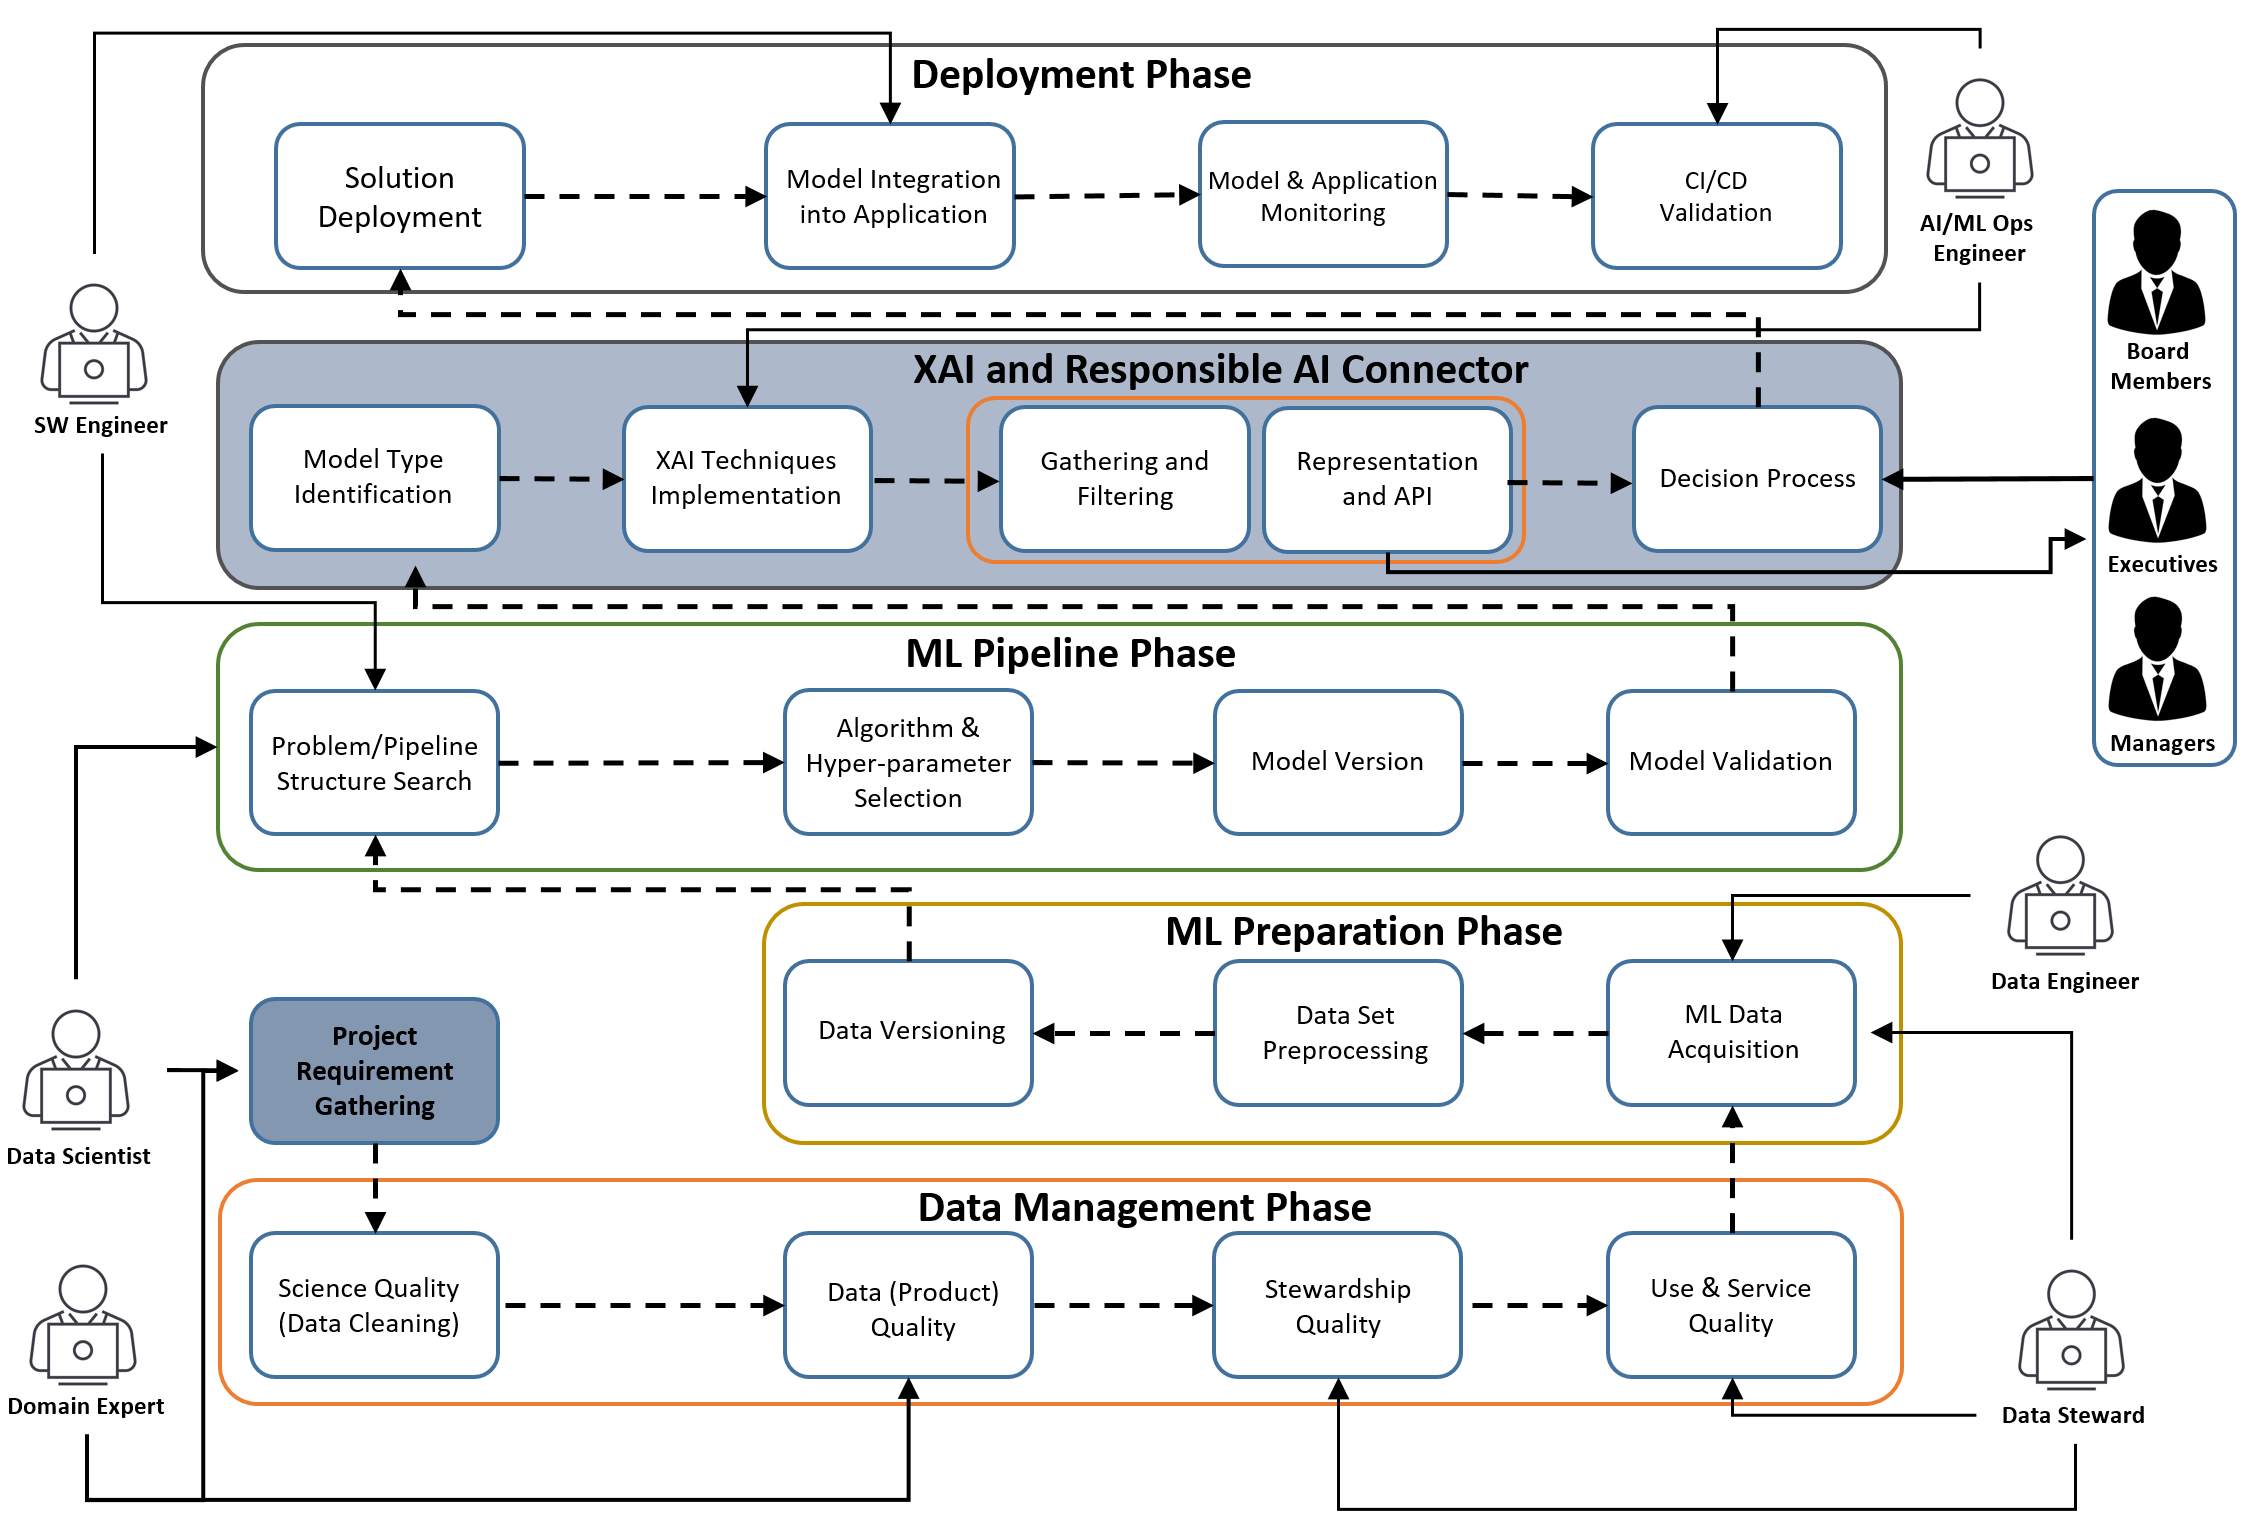
\includegraphics[width=0.8\textwidth]{ML-OPS_with_XAI.png}
	\caption{Transition from traditional to the current approach}
	\label{ReMixMatch}
\end{figure*}

\subsection{Figures and Tables}
\paragraph{Positioning Figures and Tables} Place figures and tables at the top and 
bottom of columns. Avoid placing them in the middle of columns. Large 
figures and tables may span across both columns. Figure captions should be 
below the figures; table heads should appear above the tables. Insert 
figures and tables after they are cited in the text. Use the abbreviation 
``Fig.~\ref{fig}'', even at the beginning of a sentence.

\begin{table}[htbp]
\caption{Table Type Styles}
\begin{center}
\begin{tabular}{|c|c|c|c|}
\hline
\textbf{Table}&\multicolumn{3}{|c|}{\textbf{Table Column Head}} \\
\cline{2-4} 
\textbf{Head} & \textbf{\textit{Table column subhead}}& \textbf{\textit{Subhead}}& \textbf{\textit{Subhead}} \\
\hline
copy& More table copy$^{\mathrm{a}}$& &  \\
\hline
\multicolumn{4}{l}{$^{\mathrm{a}}$Sample of a Table footnote.}
\end{tabular}
\label{tab1}
\end{center}
\end{table}


Figure Labels: Use 8 point Times New Roman for Figure labels. Use words 
rather than symbols or abbreviations when writing Figure axis labels to 
avoid confusing the reader. As an example, write the quantity 
``Magnetization'', or ``Magnetization, M'', not just ``M''. If including 
units in the label, present them within parentheses. Do not label axes only 
with units. In the example, write ``Magnetization (A/m)'' or ``Magnetization 
\{A[m(1)]\}'', not just ``A/m''. Do not label axes with a ratio of 
quantities and units. For example, write ``Temperature (K)'', not 
``Temperature/K''.

\section*{Acknowledgment}

The preferred spelling of the word ``acknowledgment'' in America is without 
an ``e'' after the ``g''. Avoid the stilted expression ``one of us (R. B. 
G.) thanks $\ldots$''. Instead, try ``R. B. G. thanks$\ldots$''. Put sponsor 
acknowledgments in the unnumbered footnote on the first page.

\section*{References}

Please number citations consecutively within brackets . The 
sentence punctuation follows the bracket . Refer simply to the reference 
number, as in ---do not use ``Ref. '' or ``reference '' except at 
the beginning of a sentence: ``Reference  was the first $\ldots$''

Number footnotes separately in superscripts. Place the actual footnote at 
the bottom of the column in which it was cited. Do not put footnotes in the 
abstract or reference list. Use letters for table footnotes.

Unless there are six authors or more give all authors' names; do not use 
``et al.''. Papers that have not been published, even if they have been 
submitted for publication, should be cited as ``unpublished'' . Papers 
that have been accepted for publication should be cited as ``in press'' . 
Capitalize only the first word in a paper title, except for proper nouns and 
element symbols.

For papers published in translation journals, please give the English 
citation first, followed by the original foreign-language citation .

\bibliographystyle{IEEEtran}
\bibliography{bibfile.bib}

\end{document}
